\section{Systematic Uncertainties and Result}
\label{sec:syst}
\emph{In short: thirteen variants in four groups, fitted by both methods on the same candidates, give $0.0070$ (Bayesian) and $0.0072$ (Frequentist), dominated by the particle-identification requirement.}
The systematic study asks how much the result depends on choices of the analysis that the data do not fix. The Frequentist and Bayesian fits share one study, so that the two uncertainties are comparable: the same thirteen variants of the nominal choices, fitted by both methods on exactly the same candidates, and the same rule to combine them. The variants (listed in Table~\ref{tab:syst}) change one choice at a time and fall in four groups: the \emph{window}, the \emph{background} model, the \emph{signal} model and the \emph{preselection} cuts.

The shift $\Delta=\Araw^{\mathrm{var}}-\Araw^{\mathrm{nom}}$ of a variant is not necessarily a systematic effect: when a variant changes the sample (window, preselection) the two samples are nested and part of $\Delta$ is a statistical fluctuation of expected size $\sigma_B=\sqrt{|\sigma_{\mathrm{var}}^2-\sigma_{\mathrm{nom}}^2|}$~\cite{barlow}, and such a variant contributes only if $|\Delta|>\sigma_B$. A variant that the data reject ($\Delta\chi^2>25$ on the same data) is excluded: this removes the single exponential ($\Delta\chi^2=134$\appref{sec:bayes_gof}). The largest remaining $|\Delta|$ of each group is its uncertainty, since the variants of a group are alternative descriptions of the same choice, and the groups, being independent choices, are added in quadrature.

\begin{table}[t]
\centering
\small
\resizebox{\ifdim\width>\linewidth\linewidth\else\width\fi}{!}{\begin{tabular}{llcc}
\toprule
Group & Variant & Bayesian & Frequentist \\
\midrule
Window & $[5050,5600]$ & $-0.0003$ ($0.0009$) & $-0.0004$ ($0.0005$) \\
 & $[5150,5600]$ & $-0.0001$ ($0.0007$) & $-0.0005$ ($0.0021$) \\
 & $[5100,5450]$ & $+0.0002$ ($0.0009$) & $-0.0001$ ($0.0003$) \\
 & $[5100,5700]$ & $-0.0014$ ($0.0010$) & $-0.0014$ ($0.0001$) \\
& \emph{group uncertainty} & $\mathit{0.0014}$ & $\mathit{0.0014}$ \\
\midrule
Background & single exponential (rejected) & $-0.0037$ & $-0.0039$ \\
 & shape shared between charges & $-0.0037$ & $-0.0040$ \\
 & symmetric, $A_b=0$ & $-0.0028$ & $-0.0031$ \\
& \emph{group uncertainty} & $\mathit{0.0037}$ & $\mathit{0.0040}$ \\
\midrule
Signal & Crystal Ball & $-0.0002$ & $-0.0006$ \\
 & $\mu,\sigma$ per charge & $-0.0000$ & $-0.0001$ \\
& \emph{group uncertainty} & $\mathit{0.0002}$ & $\mathit{0.0006}$ \\
\midrule
Preselection & $\texttt{ProbK}>0.4$ & $-0.0032$ ($0.0038$) & $-0.0032$ ($0.0037$) \\
 & $\texttt{ProbK}>0.6$ & $+0.0058$ ($0.0048$) & $+0.0058$ ($0.0050$) \\
 & $\texttt{ProbPi}<0.4$ & $+0.0022$ ($0.0022$) & $+0.0020$ ($0.0023$) \\
 & $\texttt{ProbPi}<0.6$ & $-0.0004$ ($0.0020$) & $-0.0006$ ($0.0017$) \\
& \emph{group uncertainty} & $\mathit{0.0058}$ & $\mathit{0.0058}$ \\
\midrule
\multicolumn{2}{l}{Total (quadrature)} & $0.0070$ & $0.0072$ \\
\bottomrule
\end{tabular}}
\caption{Systematic study common to the Bayesian and Frequentist fits: shift $\Delta$ of $\Araw$ for each variant and, in parentheses and for the variants that change the sample, the expected statistical spread $\sigma_B$ of the shift. The largest contributing shift of each group is its uncertainty (italics); the groups are added in quadrature. The single exponential is rejected by the data and excluded. For the window $[5150,5600]$ the Frequentist uncertainty is scaled from the number of events, since the Hesse matrix of that fit is not accurate.}
\label{tab:syst}
\end{table}

Figure~\ref{fig:syst_pid_scan} shows the scan of each particle-identification cut, with the expected spread $\sigma_B$.

\begin{figure*}[!t]
\centering
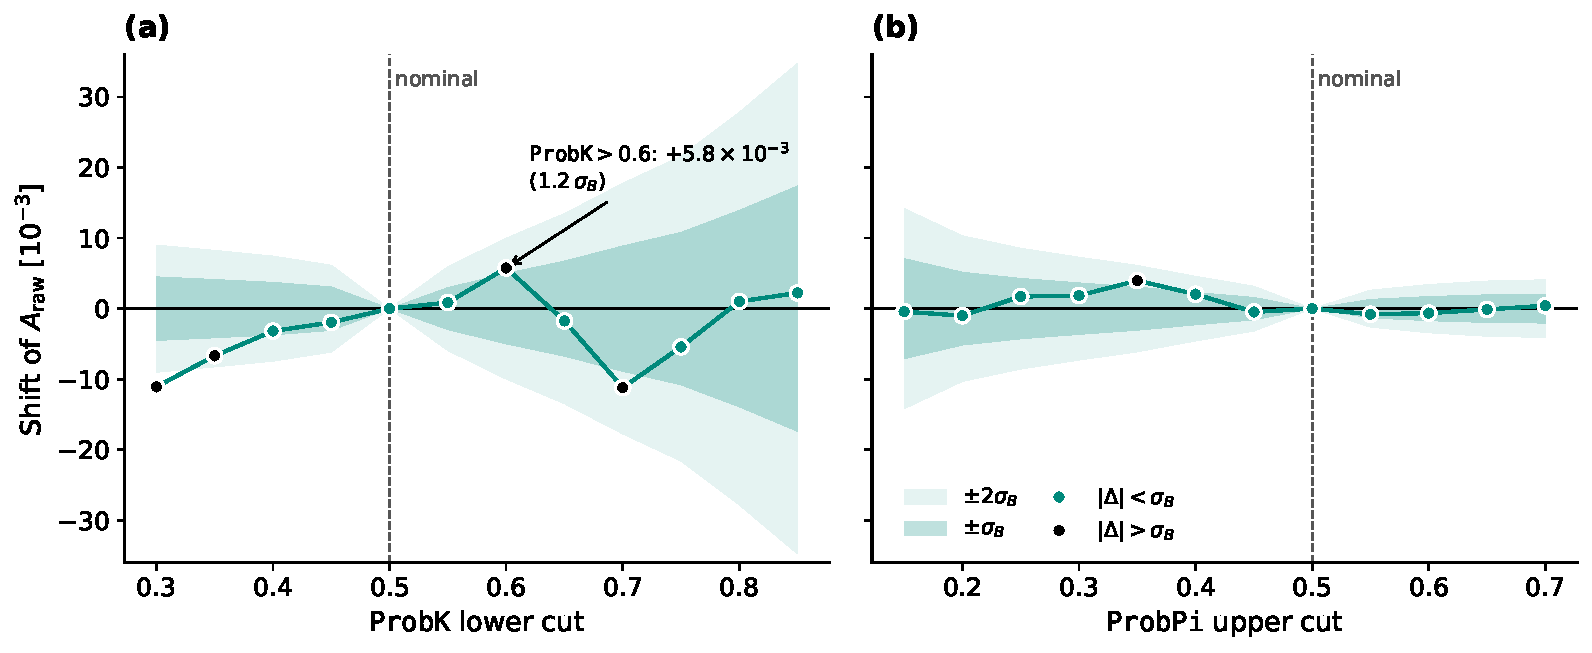
\includegraphics[width=0.85\textwidth]{figures/short_pid_scan.pdf}
\caption{Shift of $\Araw$ (Frequentist fit) as a function of (a) the $\mathtt{ProbK}$ lower cut and (b) the $\mathtt{ProbPi}$ upper cut, in steps of $0.05$, with the expected statistical spread of the nested sample ($\pm\sigma_B$ dark, $\pm2\sigma_B$ light; zero at the nominal cut, dash-dotted line). On the tight side of $\mathtt{ProbK}$ the points scatter around zero without trend and the pion requirement is flat; loosening $\mathtt{ProbK}$ moves $\Araw$ monotonically.}
\label{fig:syst_pid_scan}
\end{figure*}

The results are in Table~\ref{tab:syst}\appref{sec:syst_tables}. The two methods give the same shifts to within $\sim$$0.0005$ and the same group uncertainties, with totals of $0.0070$ (Bayesian) and $0.0072$ (Frequentist):
\begin{gather*}
\text{Bayesian:}\\ \Araw=-0.0443\pm0.0085\,(\text{stat})\pm0.0070\,(\text{syst}),\\[2pt]
\text{Frequentist:}\\ \Araw=-0.0441\pm0.0085\,(\text{stat})\pm0.0072\,(\text{syst}).
\end{gather*}

The preselection dominates, through the single variant $\texttt{ProbK}>0.6$ ($+0.0058$, $1.2\,\sigma_B$). The scan of each cut in steps of $0.05$ \appref{app:syst}shows that this value is a fluctuation: on the tight side the shifts scatter around zero within $1.3\,\sigma_B$ without a trend, whereas loosening $\texttt{ProbK}$ moves $\Araw$ monotonically, as expected if misidentified decays not in the mass model enter the sample. The nominal requirement is therefore well placed and the preselection uncertainty conservative. The background group is second, driven by the charge dependence of the background, and the window third.

\subsection{Additional Results}
\emph{The $\sigma_B$ rule.} $\sigma_B$ is the difference of two nearly equal uncertainties, so a variant at the threshold can be classified differently by the two methods without changing the result; the rule is verified by bootstrap (the spread of the shift between a sample and its tighter subsample is $\sigma_B$)\appref{sec:checks_barlow}.

\emph{Stability scans.} The Frequentist grid scans shift $\Araw$ by at most $0.0048$ over the window edges ($55$ of $80$ fits valid), $6\times10^{-5}$ over the signal region and $0.0126$ over the grid of the two PID cuts, whose samples are smaller (mean uncertainty $0.0112$)\appref{sec:freq_stab_numbers}.
